\documentclass{llncs}
\usepackage{graphicx}     
\usepackage{cite}
\usepackage{amssymb,amsmath}
\usepackage{algorithm}
\usepackage[noend]{algorithmic}
\usepackage{array}
\usepackage{color}
%\usepackage{hyperref}
%\usepackage{multirow}

\newcommand{\Acronym}[1]{\ensuremath{{\small{\texttt{#1}}}}}
\newcommand{\Symbol}[1]{\ensuremath{\mathcal{#1}}}
\newcommand{\Function}[1]{\ensuremath{{\small \textsc{#1}}}}
\newcommand{\Constant}[1]{\ensuremath{\small{\texttt{#1}}}}
\newcommand{\Var}[1]{\ensuremath{{\small{\textsl{#1}}}}}
\newcommand{\False}{\Constant{false}}
\newcommand{\True}{\Constant{true}}
\newcommand{\Null}{\Constant{null}}
\newcommand{\Name}{\Acronym{CRoPS}}
\newcommand{\Revision}[1]{\textcolor{red}{#1}}
\newcommand{\R}{\ensuremath{\mathbb{R}}}
\newcommand{\Traj}{\ensuremath{\zeta}}
\newcommand{\Tree}{\Symbol{T}}
\newcommand{\LTLNext}{\bigcirc}
\newcommand{\LTLEventually}{\Diamond}
\newcommand{\LTLAlways}{\Box}
\newcommand{\LTLUntil}{\cup}
\newcommand{\LTLRelease}{\Symbol{R}}
\newcommand{\Automaton}{\Symbol{A}}


 \begin{document}

\frontmatter
\pagestyle{headings}  
\addtocmark{} 

\mainmatter 

\title{Path Planning for Swarms by Combining Probabilistic Roadmaps and
  Potential Fields}

\author{Alex Wallar\inst{1} \and Erion Plaku\inst{2}}

\institute{
School of Computer Science, University of St Andrews, \\
St Andrews, Fife KY16 9AJ, Scotland, United Kingdom
\and
Dept. of Electrical Engineering and Computer Science\\ 
Catholic University of America, Washington DC 20064 USA
}


\maketitle
\begin{abstract}
This paper combines probabilistic roadmaps with potential
fields in order to enable a robotic swarm to effectively move to a
desired destination while avoiding collisions with obstacles and each
other. Potential fields provide the robots with local, reactive,
behaviors that seek to keep the swarm moving in cohesion and away from
the obstacles. The probabilistic roadmap provides global path planning
which guides the swarm through a series of intermediate goals in order
to effectively reach the desired destination. Random walks in
combination with adjustments to the potential fields and intermediate
goals are used to help stuck robots escape local minima.  Experimental
results provide promising validation on the efficiency and scalability
of the proposed approach. Source code is made publicly available.
\end{abstract}


\section{Introduction}
\label{sec:Intro}


Swarm robotics seeks to enable a large number of robots to accomplish
complex tasks via simple interactions with one another and the
environment \cite{reynolds1987flocks}.  Swarm robotics draws
inspiration from social insects, such as ants and bees, where
intelligent group behaviors emerge from simple interactions among the
individuals. Such framework provides a level of scalability and
robustness that is difficult to achieve with centralized
approaches. As research progresses, applications of swarm robotics are
emerging in exploration, mapping,
monitoring, inspection, and search-and-rescue missions, as surveyed in
\cite{swarm,swarmReview12}.


Fundamental to these objectives is the ability of the swarm to move in
cohesion to a goal destination while avoiding collisions with
obstacles and among the robots in the swarm. This path-planning
problem presents significant challenges. As path
planning is PSPACE-complete, exact algorithms, which always find a
solution if it exists and report no solution otherwise, are difficult
to implement and are limited in practicality to low-dimensional
systems due to the exponential dependency on the problem dimension
\cite{Rei79,Can88,SchSha88}.
As a result, research has focused on alternative approaches that do
not determine the existence of a solution but seek instead
to achieve efficiency and scalability in increasingly complex
settings.

%APFs provide
%the swarm with local, reactive, behaviors emerging from the
%combination of repulsive forces from the obstacles and the attractive
%forces from the goal.



A common approach in path planning for robotic swarms is to impose
artificial potential functions (APFs) that seek to push the swarm away
from the obstacles and toward the goal destination \cite{Khatib86,reif1999social,book:SwarmsAPFs,tanner2005formation}. APFs provide
scalability as the addition of new robots to the swarm generally
requires only computation of repulsive forces from obstacles,
attractive forces from the goal, and forces resulting from the limited
interactions with neighboring robots in the swarm.  However, an
inherent challenge with APFs is the tendency to get stuck in local
minima\footnote{APFs that avoid local minima exist in limited cases, e.g., a
point robot moving in a generalized sphere world \cite{RK92}, but
not in a general path-planning setting for swarms.}, especially when planning paths for large swarms moving in
cluttered environments and through narrow passages.  
%
%Alternative sampling-based approaches avoid the issue of local minima
%altogether by selectively sampling and exploring the configuration
%space for a collision-free path to the goal
%\cite{book:MP,book:LaValle}.

To improve the efficiency of path planning for robotic swarms, this
paper develops a novel approach, named $\Name$ (\texttt{C}ombined
\texttt{Ro}admaps and \texttt{P}otentials for \texttt{S}warms), which combines APFs
with probabilistic roadmaps (PRMs). The underlying idea in PRMs is to
capture the connectivity of the configuration space via a roadmap
obtained by sampling collision-free configurations and connecting
neighboring configurations with collision-free paths. A graph search
is then performed on the roadmap to obtain a collision-free path from
an initial to a goal configuration.  Starting with the original PRM
\cite{PRM} and continuing over the years, PRMs have had great success
in solving challenging problems
\cite{TogglePRM,UOBPRM,PlakuTRO05,HSUBridge,GaussianPRM,manocha12}.
The work in \cite{PRMapf1,PRMapf2} use APFs to increase PRM sampling near
obstacles in order to facilitate connections through narrow passages.
The work in \cite{LienSwarming,LienSwarmingRules,LienShepherding} uses
PRM to enable robotic swarms achieve different
behaviors such as homing, environment coverage, goal searching, and
shepherding. The roadmap, however, is build over the high-dimensional
configuration space, which considerably increases the computational
cost. The work in \cite{KostasSwarm} uses multi-level PRMs in
combination with Bezier curves to guide a multi-robot system to a
desired destination while maintaining a specific formation, only
breaking the formation when necessary to avoid obstacles. The approach
has been applied only to a small number of robots and requires
considerable precomputation to build the multi-level PRMs.

%Starting with the original PRM
%\cite{PRM} and continuing over the years, PRMs have had great success
%in solving challenging path-planning problems which could not be
%addressed with APFs or other approaches
%\cite{TogglePRM,UOBPRM,PlakuTRO05,HSUBridge,GaussianPRM,manocha12,PRMapf1,PRMapf2,KostasSwarm}
%(see also surveys in \cite{book:MP,book:LaValle}).  

Even though significant progress has been made, scalability still
remains problematic in PRMs \cite{book:MP,book:LaValle}. As the number
of robots increases, it becomes difficult to sample collision-free
configurations and generate collision-free paths that connect
neighboring configurations. Moreover, significantly larger roadmaps
are needed to capture the connectivity of the configuration space,
which becomes high dimensional as it corresponds to the Cartesian
product of the individual configuration spaces.  As a result,
efficiency of PRMs starts deteriorating as the number of robots is
increased. These issues become even more problematic when considering
robotic swarms since PRMs do not have a mechanism to ensure that the
robots move in cohesion as a swarm rather than as individual entities.

While the proposed approach $\Name$ draws from PRM the underlying idea
of using a roadmap, it does not suffer from scalability issues as the
roadmap is constructed over the two-dimensional workspace instead of
the high-dimensional configuration space of the swarm. Moreover,
$\Name$ does not use the roadmap to plan the entire path of the swarm,
but rather to generate a series of intermediate goals that serve as
attractive potentials to guide the swarm toward the desired
destination. $\Name$ then relies on APFs to enable the robots move in
cohesion as a swarm from one intermediate goal to the other while
avoiding collisions. This combination of probabilistic roadmaps with
APFs is crucial to the efficiency and scalability of the proposed
approach. Experimental results in simulation with increasingly large
swarms moving in complex environments containing numerous obstacles
and narrow passages provide promising validation.

%
%\subsubsection{Related Work:}
%We refer the reader to \cite{book:SwarmsAPFs,swarmReview12} for
%extensive reviews on swarm robotics. The discussion below focuses on
%closely related approaches that rely on PRMs and APFs.

%%PRMs in combination with APFs have been used before
%%in different contexts. 
%The work in \cite{PRMapf1} uses APFs obtained from partial solutions
%of Laplace's equation to increase the sampling of PRM nodes near
%obstacles in order to facilitate connections through narrow
%passages. Follow-up work \cite{PRMapf2} simplified the computation by
%developing a particular family of potential functions suitable for
%increasing sampling in narrow passages. These approaches, however,
%have not been applied to path planning for robotic swarms and have
%similar limitations on scalability as the traditional PRM approaches.

%The work in \cite{LienSwarming,LienSwarmingRules,LienShepherding} uses
%probabilistic roadmaps to enable robotic swarms
%achieve different behaviors such as homing, environment coverage, goal
%searching, and shepherding. The roadmap, however, is build over the
%high-dimensional configuration space, which considerably increases the
%computational cost.

%The work in \cite{KostasSwarm} uses multi-level roadmaps in
%combination with Bezier curves to guide a multi-robot
%system to a desired destination while maintaing a specific formation,
%only breaking the formation when necessary to avoid obstacles. The
%approach has been applied only to a small number of robots (up to
%five) and requires considerable precomputation to build the
%multi-level roadmaps.

 



\section{Method}
\label{sec:Method}

%$\Name$ combines probabilistic roadmaps with APFs in order
%to enable a swarm of robots to effectively move to a desired
%destination while avoiding collisions with obstacles and each other.
%The probabilistic roadmap provides global path planning to determine
%appropriate intermediate goals for the swarm. The potential
%fields provide local planning to enable the robots move together as a swarm
%towards the goal while avoiding collisions. More specifically, 
%

The swarm motions are governed by the following criteria:
\begin{enumerate}
\item There is long range attraction to intermediate goals and final destination. 
\item Robots are repulsed from obstacles.
\item Robots move as a swarm while keeping some separation from one another.
\item A robot's heading is influenced by the headings of its neighbors.
\end{enumerate}
To guide the swarm to the final destination, global path planning
based on probabilistic roadmaps is used to determine suitable
intermediate goals. The roadmap is constructed by sampling
collision-free points and connecting neighboring points with
collision-free edges to obtain a graph that captures the connectivity
of the environment. Roadmap vertices and edges are associated with
weights that estimate the feasibility of the swarm to pass through
their surrounding areas. The shortest path in the roadmap to the final
destination is used to provide a series of intermediate goals that the
swarm can follow to effectively reach the final destination. An
attractive potential, denoted as $PF_\Var{igoal}(b)$, is added between
each robot $b$ and its current intermediate goal. When the robot reaches the
current intermediate goal, the next point in the shortest path is set
as the new intermediate goal.

To avoid collisions with obstacles, $\Name$ creates a strong repulsive potential
field, denoted as $PF_\Var{obst}(b)$, which
pushes each robot $b$ away from the obstacles. The repulsive potential
increases quadratically with respect to the inverse of the distance
from the robot to the obstacles. Such rapid increase prevents the robots
from getting too close to the obstacles. 

To maintain separation among the robots in the swarm, each robot is
pushed away from its neighbors. A weak sigmoidal repulsive
potential, denoted as $PF_\Var{sep}(b)$, is employed rather than a
strong quadratic repulsive potential in order to push $b$ away
from its neighbors but not so strongly as to separate it from the
swarm.

To move as a swarm, a robot's heading is influenced by the headings of
its neighbors, defined as $PF_\Var{heading}(b)$. To promote effective
movements, preference is given to neighbors that are not
stuck and are neither too close nor too far. The headings of the
neighbors that are chosen are averaged and combined with the other
potential fields to determine the new heading and position of each
robot.



\begin{algorithm}[t]
\caption{Pseudocode for $\Name$}
\label{algo:Main}
\begin{algorithmic}[1]
\setcounter{ALC@line}{0}
%\COMMENT{generate $n$ additional roadmap vertices}
\vspace*{1mm}
\STATE $RM = (V, E) \leftarrow \Function{ConstructRoadmap}()$, where
\STATE \hspace*{5mm} $V \leftarrow$ sample numerous random points, discard those that are in collision 
\STATE \hspace*{5mm} $E \leftarrow$ connect neighboring points in $V$,
discard those edges that are in collision
\STATE \hspace*{5mm} $w(q_i) \leftarrow$ assign weight to each vertex $q_i \in V$
\STATE \hspace*{5mm} $w(q_i, q_j) \leftarrow$ assign weight to each edge $(q_i, q_j) \in E$
\STATE $\zeta = [q_k]_{k=1}^m \leftarrow
\Function{IntermediateGoals}(RM)$ \hfill{\emph{$\diamondsuit$ obtained from shortest path}}
\STATE $\Var{igoal}(b) \leftarrow \zeta(1)$
\hfill{\emph{$\diamondsuit$ set current intermediate goal for each
    robot}}

\WHILE{$\Function{solved}() = \False$}
\FOR{$b \in \Var{Robots}$ with $\Function{ReachedIntermediateGoal}(b) =\True$} 
\STATE $\Var{igoal}(b) \leftarrow \Function{NextIntermediateGoal}(\zeta)$
\ENDFOR

\FOR{$b \in \Var{Robots}$ }
\STATE $PF(b) \leftarrow \Function{superimpose}(PF_\Var{obst}(b),
PF_\Var{sep}(b), PF_\Var{igoal}(b), PF_\Var{heading}(b), PF_\Var{escape}(b))$
\STATE $\Var{NewHeading}(b) \leftarrow w_1 \Var{heading}(b) + w_2 PF(b)$
\ENDFOR

\FOR{$b \in \Var{Robots}$ }
\STATE $\Var{heading}(b) \leftarrow \Var{NewHeading}(b)$; $\quad$ 
$\Var{pos}(b) \leftarrow \Var{pos}(b) + \Var{heading}(b)$
\ENDFOR
\ENDWHILE


\end{algorithmic}
\end{algorithm}




The different potential fields are superimposed to obtain the overall
force vector applied to each robot $b$. In this way, the potential
field on the robot $b$ exerts a strong repulsive potential away from
the obstacles while attracting it to the current intermediate goal,
maintaining a separation distance from the other robots, and adjusting
the heading so that the robots move as a swarm toward the final
destination. If a robot gets stuck in local minima, random walks in
combination with adjustments to the potential fields and intermediate
goals are used to help it escape.  Pseudocode for the
overall approach is given in Algo.~\ref{algo:Main}. Details of the
main steps follow.

\subsection{Roadmap Construction}
\label{sec:RM}

 $\Name$ constructs a roadmap in order to effectively guide the swarm
toward the goal. Since the swarm could have many robots, the roadmap
is not constructed over the high-dimensional configuration
space, as it is often the case in PRM approaches, but is instead
constructed over the low-dimensional workspace where the swarm
moves. As explained in this section, $\Name$ uses the roadmap to find
intermediate areas in which the swarm can move to effectively reach
the goal.

\subsubsection{Roadmap Vertices:}
The roadmap is constructed by first sampling a large number of points
uniformly at random inside the workspace boundaries and then
discarding all the points that are in collision or too close to an
obstacle. A parameter, $d_\Var{clear}$, determines the minimum
acceptable distance from a sampled point to the nearest obstacle. The
remaining points, which are all at least $d_\Var{clear}$ units away
from the obstacles, are added as vertices to the roadmap graph $RM =
(V, E)$. A roadmap vertex $q_i$ and the clearance $d_\Var{clear}$
conceptually define a clearance area as a disk centered at $q_i$ with
radius $d_\Var{clear}$, denoted as $\Var{area}(q_i)$. In order to bias
the swarm movements toward less cluttered areas, each roadmap vertex
$q_i$ is associated with a weight $w(q_i)$ which estimates how
feasible it is for the swarm to travel through $\Var{area}(q_i)$. More
specifically, the weight is defined as
$$
w(q_i) = \left(\sum_{o \in \Var{Obstacles}} \Var{dist}(q_i, o)\right)^3,
$$ where $\Var{dist}(q_i, o)$ denotes the minimum distance from $q_i$
to the obstacle $o$. In this way, small weights indicate the presence
of obstacles nearby, which may make it more difficult for the swarm to
pass through.  As explained later in the section, $\Name$ gives
preferences to roadmap vertices associated with high weights which are
indicative of areas with high clearance. Note that other definitions
for the weight function are possible. The particular function used in
this paper worked well for the experiments as it captures the desired
properties of biasing the swarm movements towards less cluttered
areas.

\subsubsection{Roadmap Edges:}
After generating roadmap vertices, $\Name$ connects each
roadmap vertex to its $k$ nearest neighbors. Edges that are in
collision are discarded. The weight of an edge connecting $q_i$ to
$q_j$ is defined as
$$
w(q_i, q_j) = ||q_i, q_j||_2 / \min(w(q_i), w(q_j)),
$$
where $||q_i, q_j||_2$ is the Euclidean distance from $q_i$ to $q_j$. Note
that $w(q_i, q_j)$ is small when $q_i$ and $q_j$ are close to each
other and away from obstacles.

%$s_\Var{edge}$ is a scaling constant to account for the workspace dimensions and

\subsubsection{Intermediate Goals along Shortest Roadmap Path:} Dijkstra's shortest-path
algorithm is used to compute the shortest path $\zeta$ in the roadmap
to the final destination, where the weight of a roadmap edge $(q_i, q_j)$ is
defined by $w(q_i, q_j)$ as described above. Each vertex $q_k \in
\zeta$ defines an intermediate goal for the swarm. More specifically,
$\Name$ seeks to move the swarm to the goal by passing through the
areas $\Var{area}(q_k)$ as defined by the vertices $q_k$ along the
shortest path $\zeta$. Note that the dependency of the edge weights
on vertex weights ensures that the shortest path in the roadmap does
not come too close to the obstacles, which could lead the swarm to
often get stuck in local minima.

\subsection{Potential Fields}
\label{sec:PF}

\subsubsection{Repulsion from Obstacles:}
\label{sec:PFobst} An imperative objective for
the swarm is to always avoid collisions with obstacles. For this
reason, a repulsive potential is defined that pushes the robots away
from the obstacles. More specifically, the repulsive potential between
a robot $b$ and an obstacle $o$ is defined as
$$ P_\Var{obst}(b, o) = \frac{1}{(\Var{dist}(\Var{pos}(b), o) - \Var{radius}(b))^2},
$$ where $\Var{pos}(b)$ and
$\Var{radius}(b)$ denote the position and radius of the robot $b$, respectively. Note that the
important aspect of this repulsive function is that its value
increases rapidly as the robot approaches an obstacle. This ensures
that the robot would be pushed away and never collide with an obstacle.

%$$ P_\Var{obst}(b, o) = \frac{s_\Var{obst}\,
%  \Var{radius}(b)}{(\Var{dist}(\Var{pos}(b), o) - \Var{radius}(b))^2},
%$$ where $s_\Var{obst}$ denotes a scaling constant and $\Var{pos}(b),
%\Var{radius}(b)$ denote the robot position and radius. Note that the
%important aspect of this repulsive function is that its value
%increases rapidly as the robot approaches an obstacle. This ensures
%that the robot would be pushed away and never collide with an obstacle.

In order to limit the influence of the obstacles that are far away,
the repulsion is computed only from those obstacles that are within a
certain distance $\Delta_\Var{obst}$ from the robot. The potential
field imposed by the obstacles is then defined as 
$$
PF_\Var{obst}(b) = \sum_{\stackrel{o \in
    \Var{Obstacles}}{\Var{dist}(b, o) \leq \Delta_\Var{obst}}} (\Var{pos}(b)
- \Var{ClosestPoint}(o, \Var{pos}(b))) P_\Var{obst}(b, o),
$$
where $\Var{ClosestPoint}(\Var{pos}(b), o)$ denotes the closest point on the
obstacle $o$ to $\Var{pos}(b)$.

\subsubsection{Repulsion from other Robots:}
\label{sec:PFrobots} As the swarm moves,
the robots need to avoid coming too close to each other as it
could lead to collisions. At the same time, the robots should not be
far away from each other in order to move as a swarm. To achieve these
objectives, $\Name$ uses a weak repulsive sigmoid function
$$
P_\Var{sep}(b_i, b_j) = \frac{1}{1 +
  \exp(\delta_\Var{sep}\, ||\Var{pos}(b_i), \Var{pos}(b_j)||_2)},
$$
where $\delta_\Var{sep}$ is a scaling constant.
In order to limit the influence of the robots that are far away,
similar to the potential field for obstacles,
the repulsion is computed only from those robots that are within a
certain distance $\Delta_\Var{sep}$. The potential
field imposed on the robot $b$ by the other robots is then defined as 
$$
PF_\Var{sep}(b) = \sum_{\stackrel{b_i \in
    \Var{Robots} - \{b\}}{\Var{dist}(b, b_i) \leq \Delta_\Var{sep}}} (\Var{pos}(b)
- \Var{pos}(b_i)) P_\Var{sep}(b, b_i).
$$
In this way, the robots travel close together but are
pushed away when the come too close to one another.

\subsubsection{Attraction to the Current Intermediate Goal:}
\label{sec:PFigoal} As
discussed, $\Name$ uses the shortest path $\zeta$ in the roadmap to
set the intermediate goals for the swarm. Let $\Var{igoal}(b)$ denote
the current intermediate goal of the robot $b$. Note that
$\Var{igoal}(b)$ is associated with some point $q_k$ in $\zeta$. An
attractive potential field that
pulls the robot $b$ towards $\Var{igoal}(b)$ is then defined as 
$$
PF_\Var{igoal}(b) = \frac{\Var{igoal}(b) - \Var{pos}(b)}{1 +
  \exp(\delta_\Var{igoal}\, ||\Var{pos}(b), \Var{igoal}(b)||_2)},
$$ where $\delta_\Var{igoal}$ is a scaling constant. Although other
definitions are possible, the sigmoid function allows the robots to
reach the goal without getting too greedy, which could lead to getting
stuck in local minima. When $b$ reaches $\Var{igoal}(b)$, the next
point $q_{k+1}$ in the shortest path $\zeta$ is set as the new
intermediate goal for $b$.

\subsubsection{Influence of Neighbors on Heading:}
\label{sec:PFheading}
 In order to make
the robots move as a swarm, the heading of a robot $b$ is also
influenced by the headings of neighboring robots. In order to select
suitable neighbors, robots that are stuck
are excluded from consideration. Moreover, preference is given to those
neighbors that are neither too far nor too close from $b$. This is
achieved by using a Gaussian function $\gamma(b, b_i)$ with mean $\mu$ and standard
deviation $\sigma$, i.e.,
$$
\gamma(b, b_i) = \exp\left(\frac{-(||\Var{pos}(b), \Var{pos}(b_i)||_2 - \mu)^2}
{2\sigma^2}\right),
$$
and selecting as $\Var{Neighs}(b)$ the $k$ closest nonstuck robots
according to $\gamma(b, b_i)$.
The potential
field imposed on the robot $b$ by the headings of the neighboring robots
is then defined as
$$
PF_\Var{heading}(b) = \sum_{b_i \in
    \Var{Neighs}(b)} \Var{heading}(b_i).
$$




\subsubsection{Escaping Local Minima:}
\label{sec:PFrand}
Each robot $b$ keeps track of its past positions in order to determine
if it is stuck in local minima. More specifically, a robot $b$ is
considered stuck if it has moved very little during the last $\ell$
time steps, i.e.,
$$
\Var{stuck}(b) = 
\begin{cases}
1, & \mbox{ if } ||\Var{pos}(b) - \Var{prev}_{\ell}(b)||_2 <
\Delta_\Var{stuck}\\
0, & \mbox{ otherwise,}
\end{cases}
$$
 where $\Var{prev}_{\ell}(b)$ denotes the position of the robot 
 $\ell$ steps in the past,  and $\Delta_\Var{stuck}$ is a
 threshold constant.

If a robot $b$ is determined to be stuck, then a random vector is added
to the mix of the potential fields, i.e.,
$$
PF_\Var{escape}(b) = \Var{stuck}(b) (r_x, r_y),
$$
where $r_x, r_y$ constitute a random direction. Note that
$PF_\Var{escape}(b) = (0, 0)$ if the robot is not stuck. By performing a random walk for
several steps, the robot increases the likelihood of escaping local
minima.

In addition, when $\Var{stuck}(b) = \True$, a different mean
$\mu_\Var{stuck}$ and a different standard deviation
$\sigma_\Var{stuck}$ are used to compute
$\Var{PF}_\Var{heading}(b)$. The new mean and standard deviation have
smaller values in order to select more nearby neighbors (recall that
only nonstuck neighbors are considered for the selection.)  This
allows the robot to select different neighbors to influence its
heading, since the original neighbors could have contributed to the robot being
stuck in the local minima.

To further increase the likelihood of escaping local minima, $\Name$
also adjusts the intermediate goals of a stuck robot. In
particular, if $q_k$ is the current intermediate goal, then $\Name$
changes it to $q_{k-1}$ if the robot is still in a local minima after a
few iterations.  If the robot is still unable to escape the local
minima, the intermediate goal is set to $q_{k+1}$. By switching from
the current to a past or to a future intermediate goal, the robot is
given further flexibility which facilitates escaping local minima.


\subsubsection{Superimposition of Potential Fields:}
\label{sec:All}
The different potential fields are superimposed to obtain the overall force
vector applied to the robot $b$: 
%\begin{eqnarray*}
%PF(b) &= &||PF_\Var{obst}(b)|| PF_\Var{obst}(b) +
%        ||PF_\Var{sep}(b)|| PF_\Var{sep}(b) +
%        ||PF_\Var{igoal}(b)|| PF_\Var{igoal}(b) +\\
%      && ||PF_\Var{heading}(b)|| PF_\Var{heading}(b) +
%       w_\Var{escape}(b) PF_\Var{escape}(b),
%\end{eqnarray*}
%or
% Alex's edit
$$
PF(b) = \frac{\sum_{\phi \in \Var{fields}} \left(|| PF_\phi(b)||_2
  PF_\phi(b)\right)}{\sum_{\phi \in \Var{fields}} || PF_\phi(b)||_2},
$$
where $\Var{fields} = \{\Var{obst}, \Var{sep}, \Var{igoal},
\Var{heading}, \Var{escape}\}$.
%where $w_\Var{obst}(b), w_\Var{sep}(b), w_\Var{igoal}(b),
%w_\Var{heading}(b), w_\Var{escape}(b)$ are used to adjust the influence of the respective
%potential fields. 
The heading and the position of the robot $b$ are then updated as
\begin{eqnarray*}
\Var{heading}(b) &\leftarrow& w \Var{heading}(b) + PF(b)\\
\Var{pos}(b) &\leftarrow& \Var{pos}(b) + \Var{heading}(b),
\end{eqnarray*}
where $w$ is an adjustment constant. 

The calculation of $PF(b)$ ensures that the subfield that has the
highest potential during the current iteration will have the highest
influence when the heading is calculated. The overall potential has a
sigmoidal attraction to the immediate goal and sigmoidal repulsion
from the robots as well as an inverse distance squared repulsion from
obstacles. In this way, the potential field on the robot $b$ exerts a
strong repulsive potential away from the obstacles while attracting it
to the current intermediate goal, maintaining a separation distance
from the other robots, and adjusting the heading so that the robot $b$
moves in a direction similar to its neighbors. Escape strategies are
also applied in order for the robot to avoid getting stuck in local
minima.


\section{Experiments and Results}
\label{sec:ExpResults}

Experiments are conducted in simulation using different scenes and an
increasing number of robots to test the efficiency and scalability of
the approach. Fig.~\ref{fig:Scenes} provides an illustration of the
scenes. These scenes provide challenging test cases as the swarm has
to avoid numerous obstacles and pass through multiple narrow passages
in order to reach the final destination.

\begin{figure}
\begin{tabular}{cc}
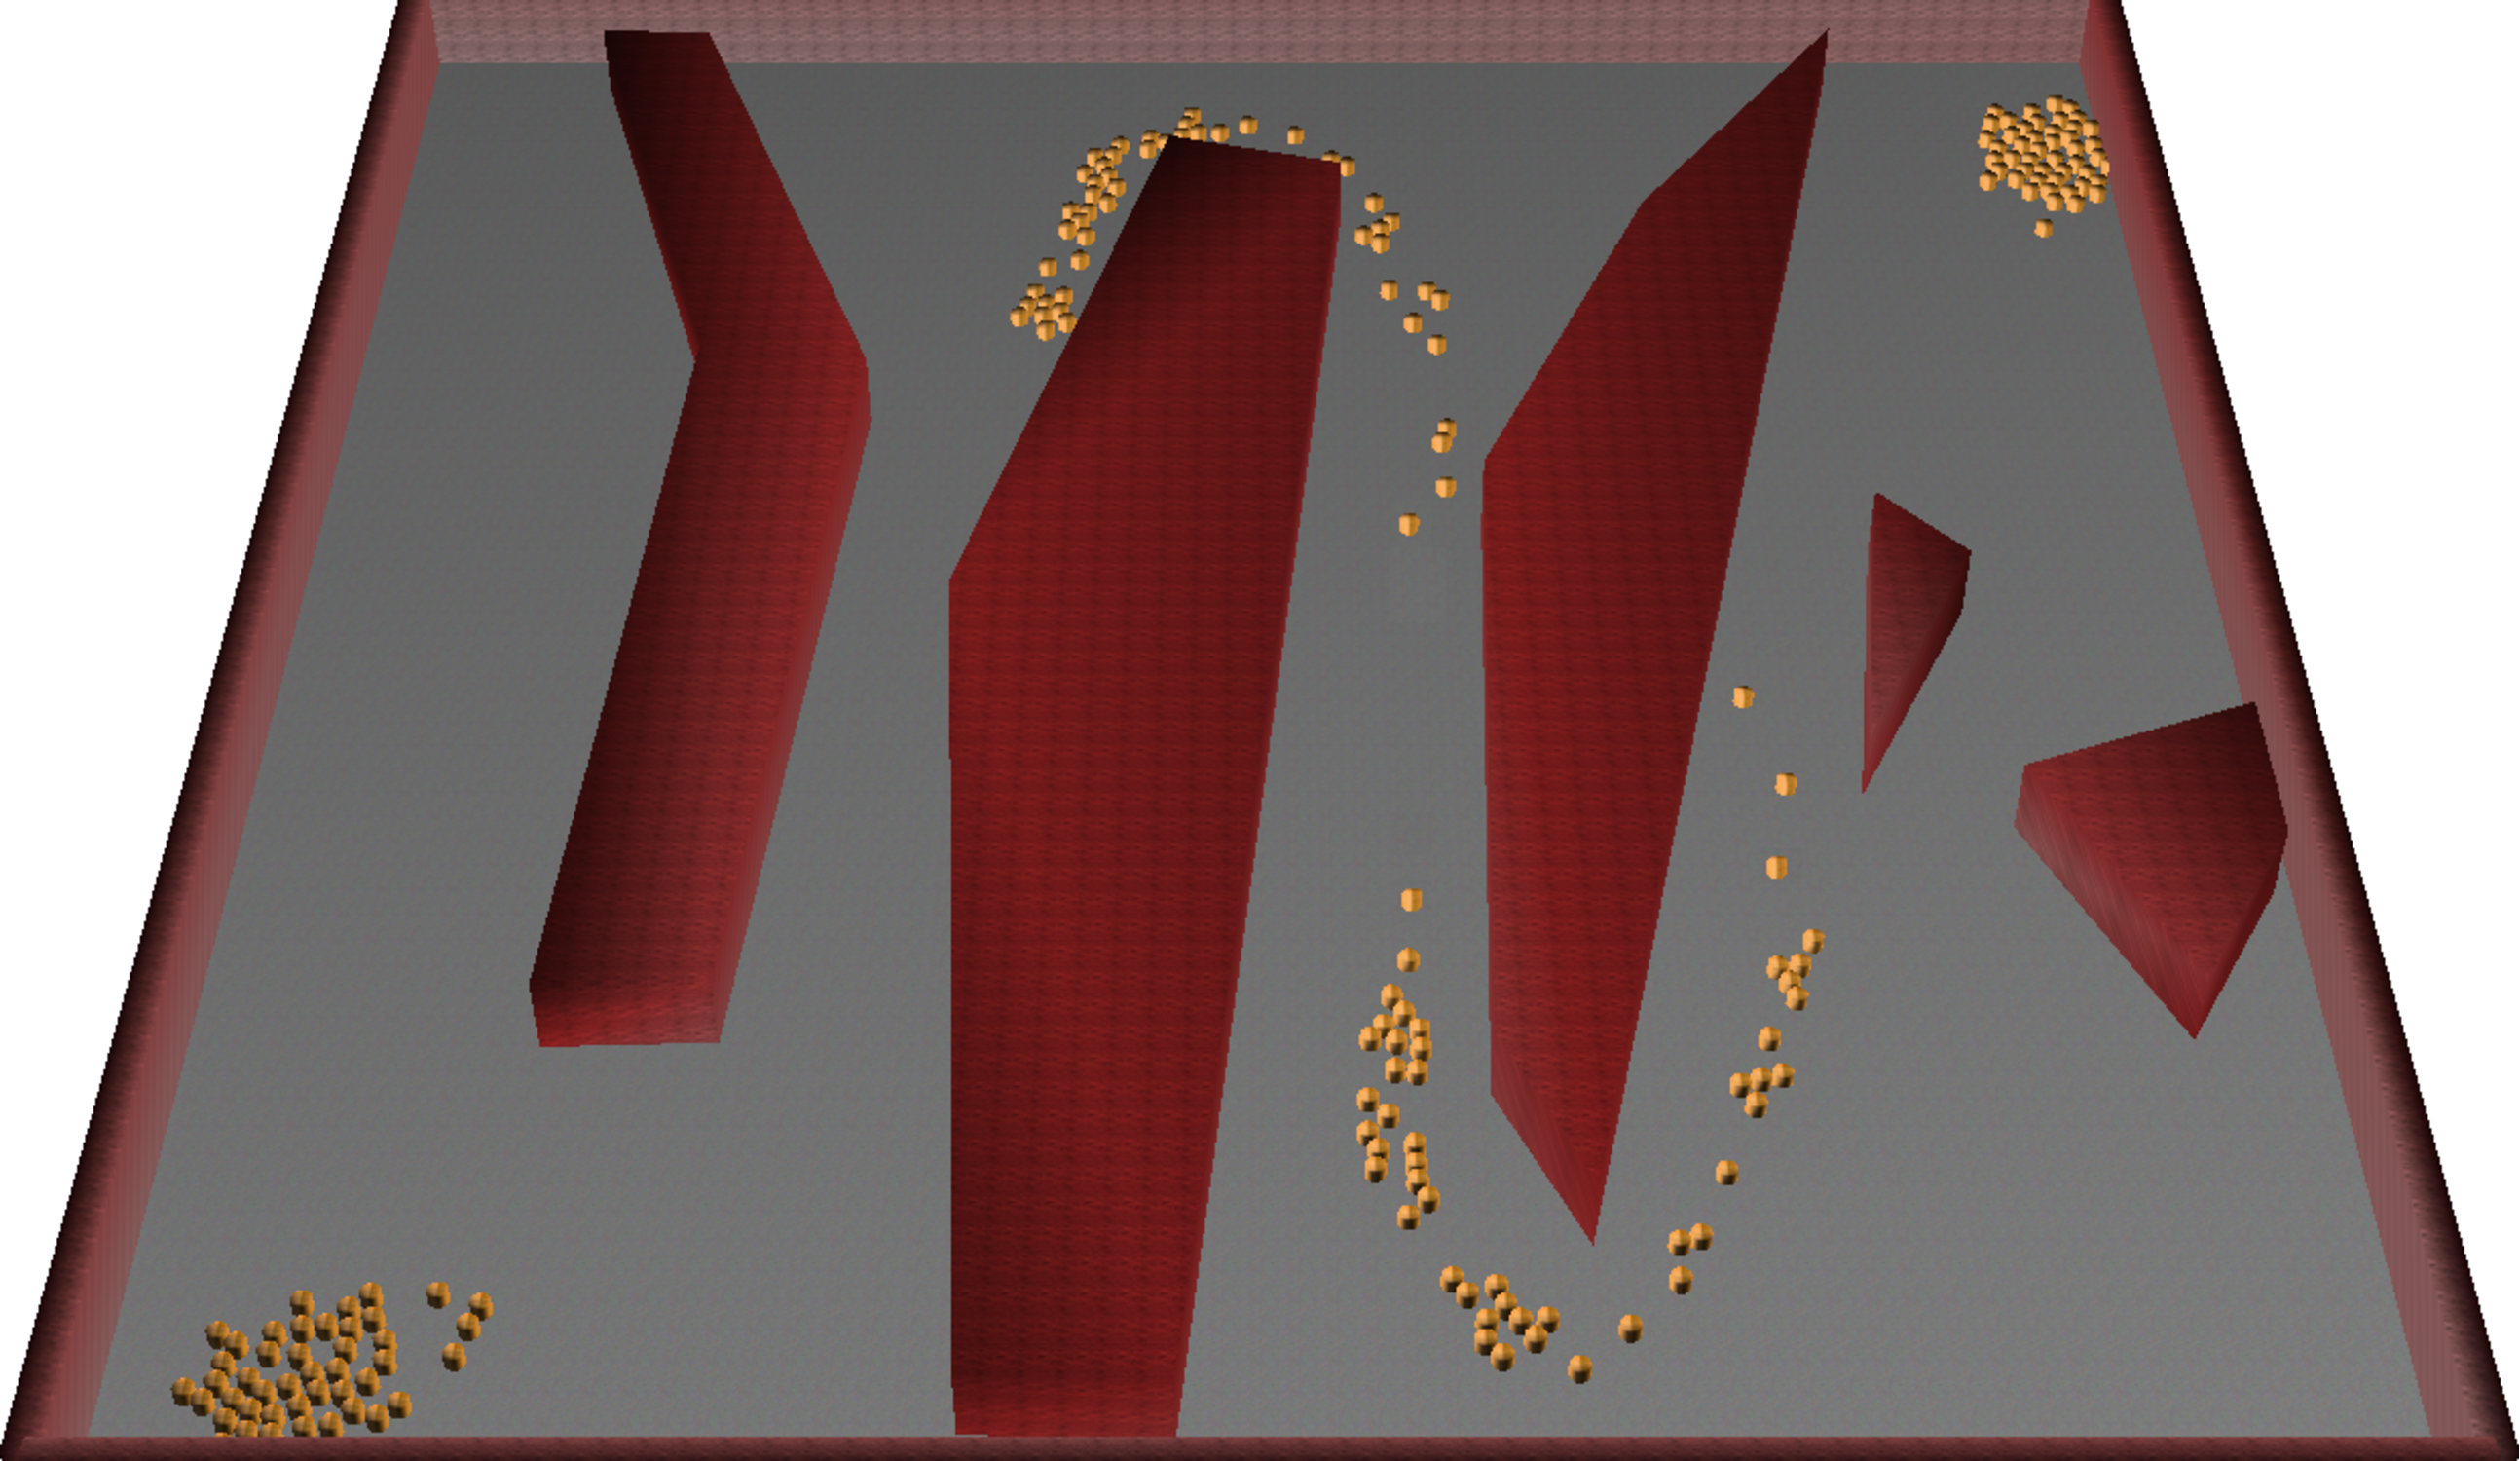
\includegraphics[width=0.55\textwidth]{m7}&
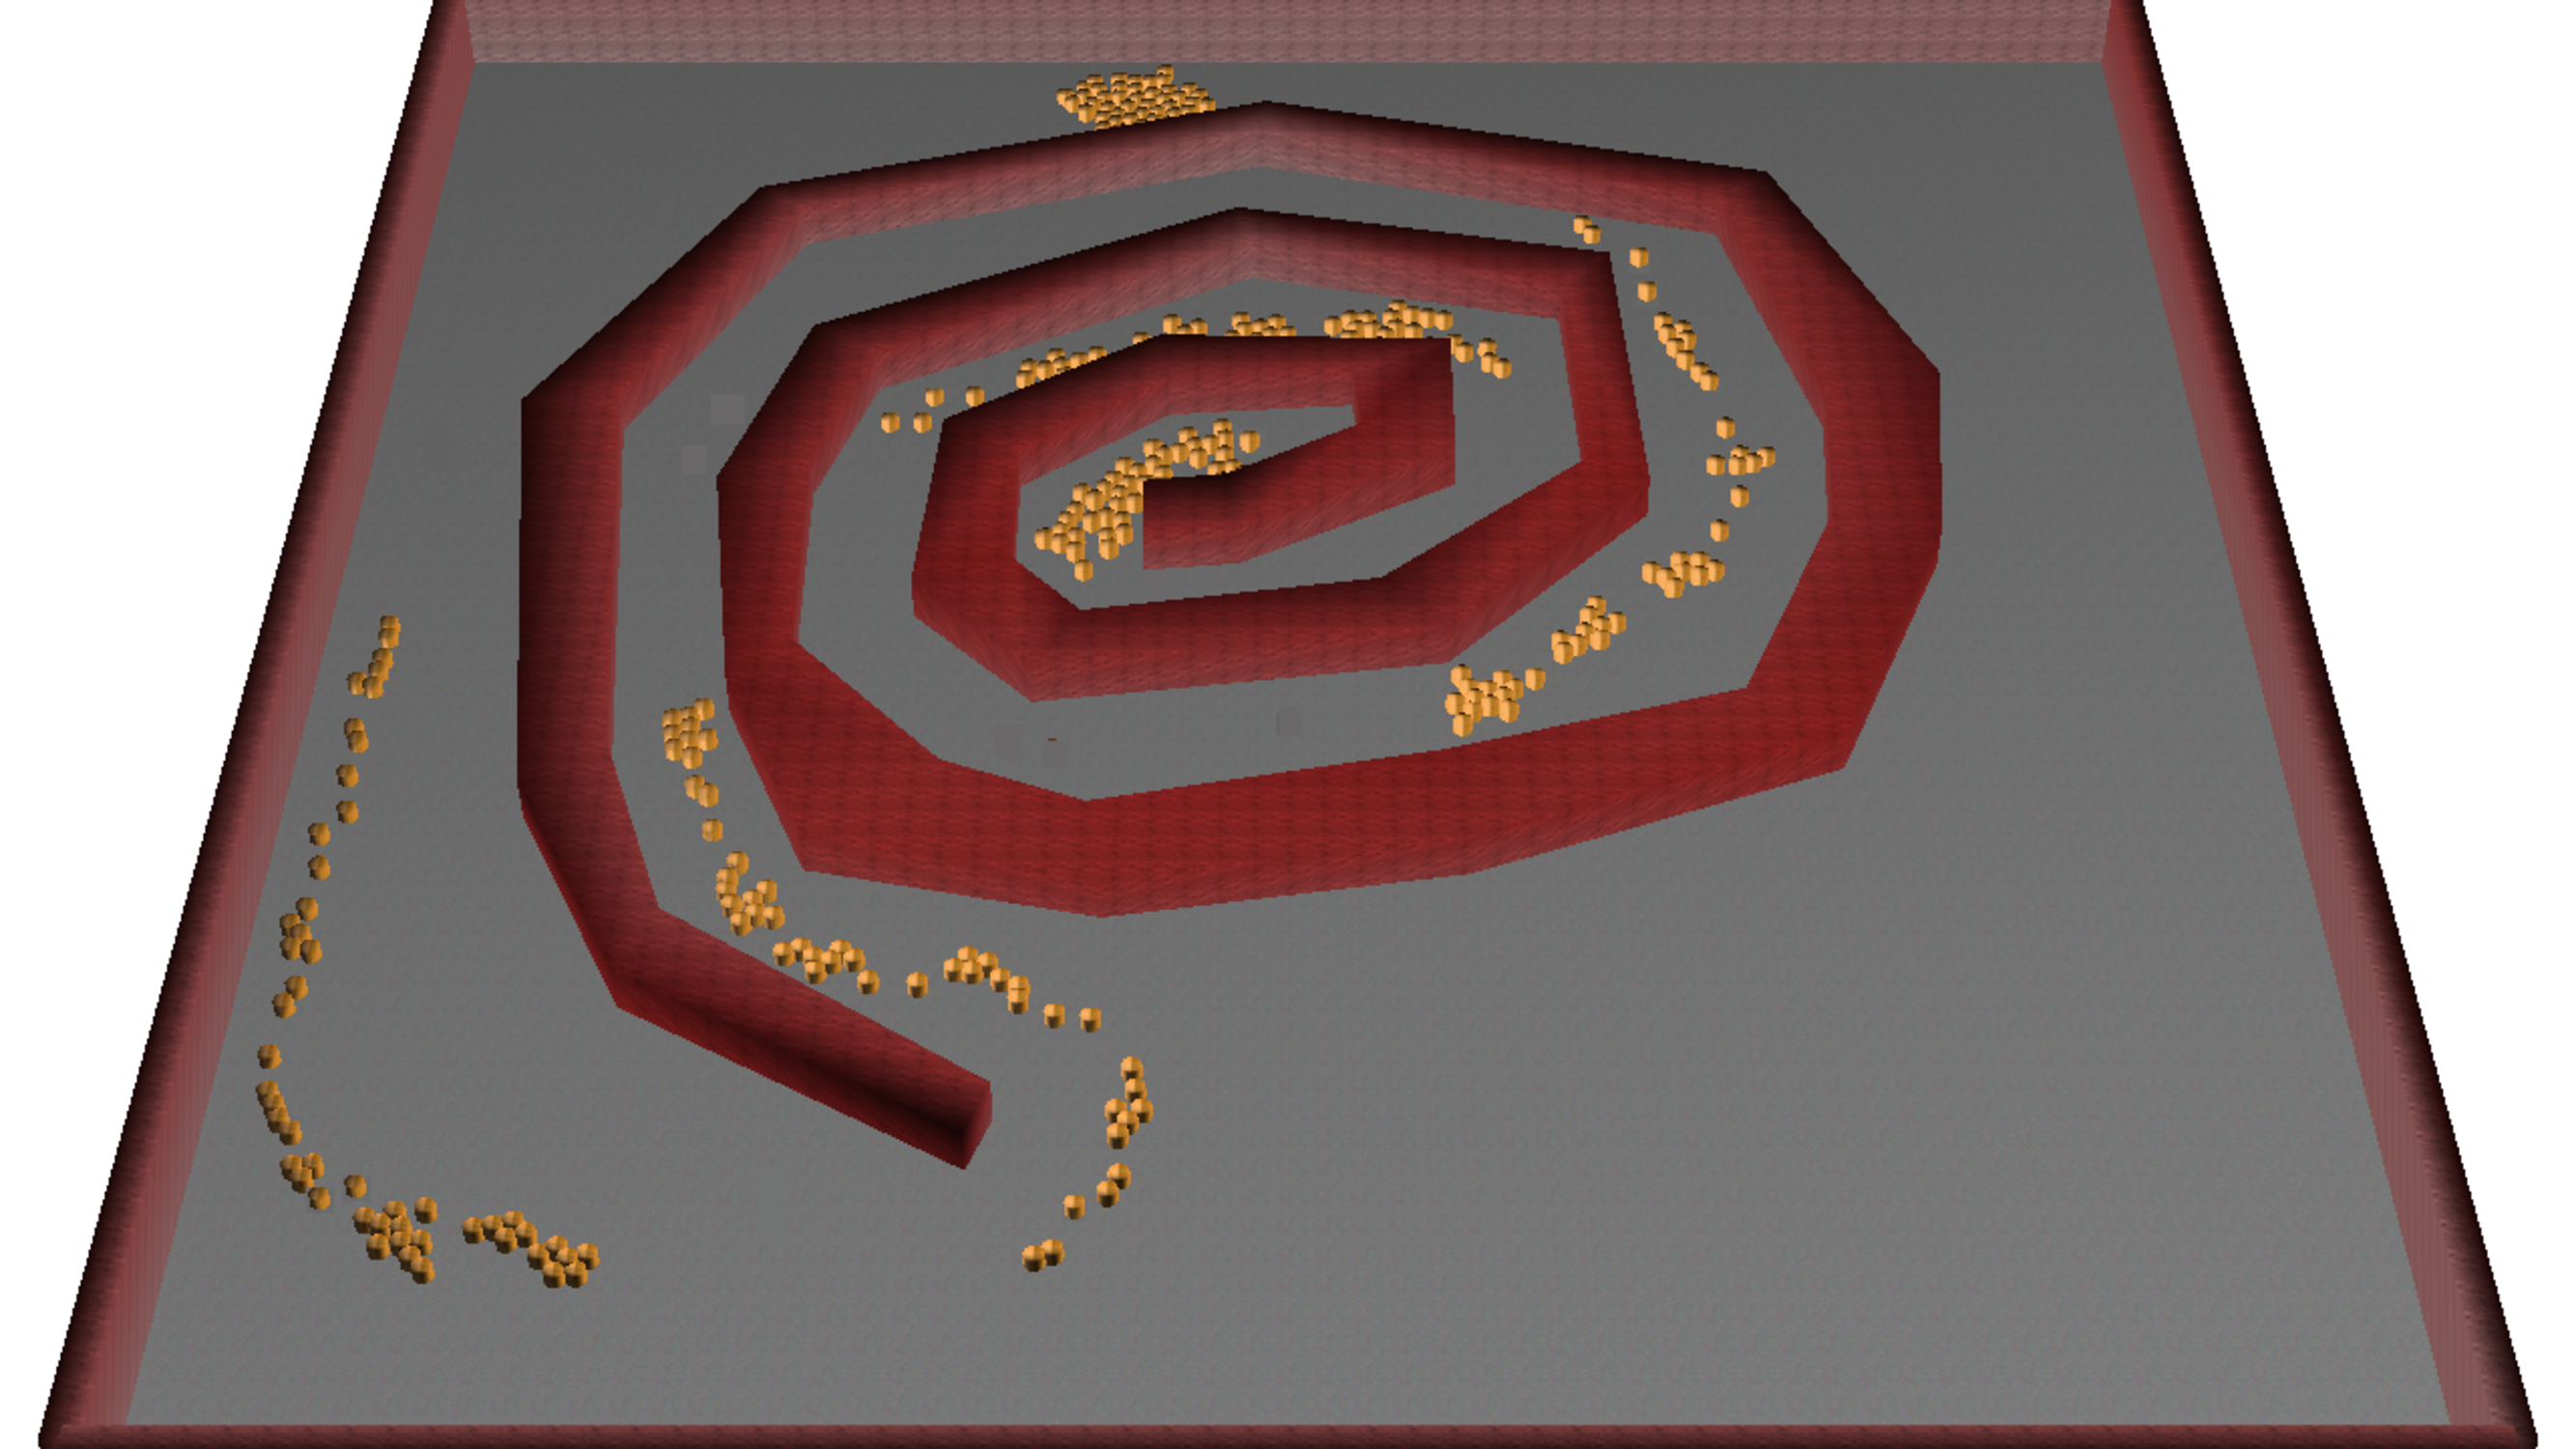
\includegraphics[width=0.55\textwidth]{scene1}\\
(a) scene1 & (b) scene2\\
\multicolumn{2}{c}{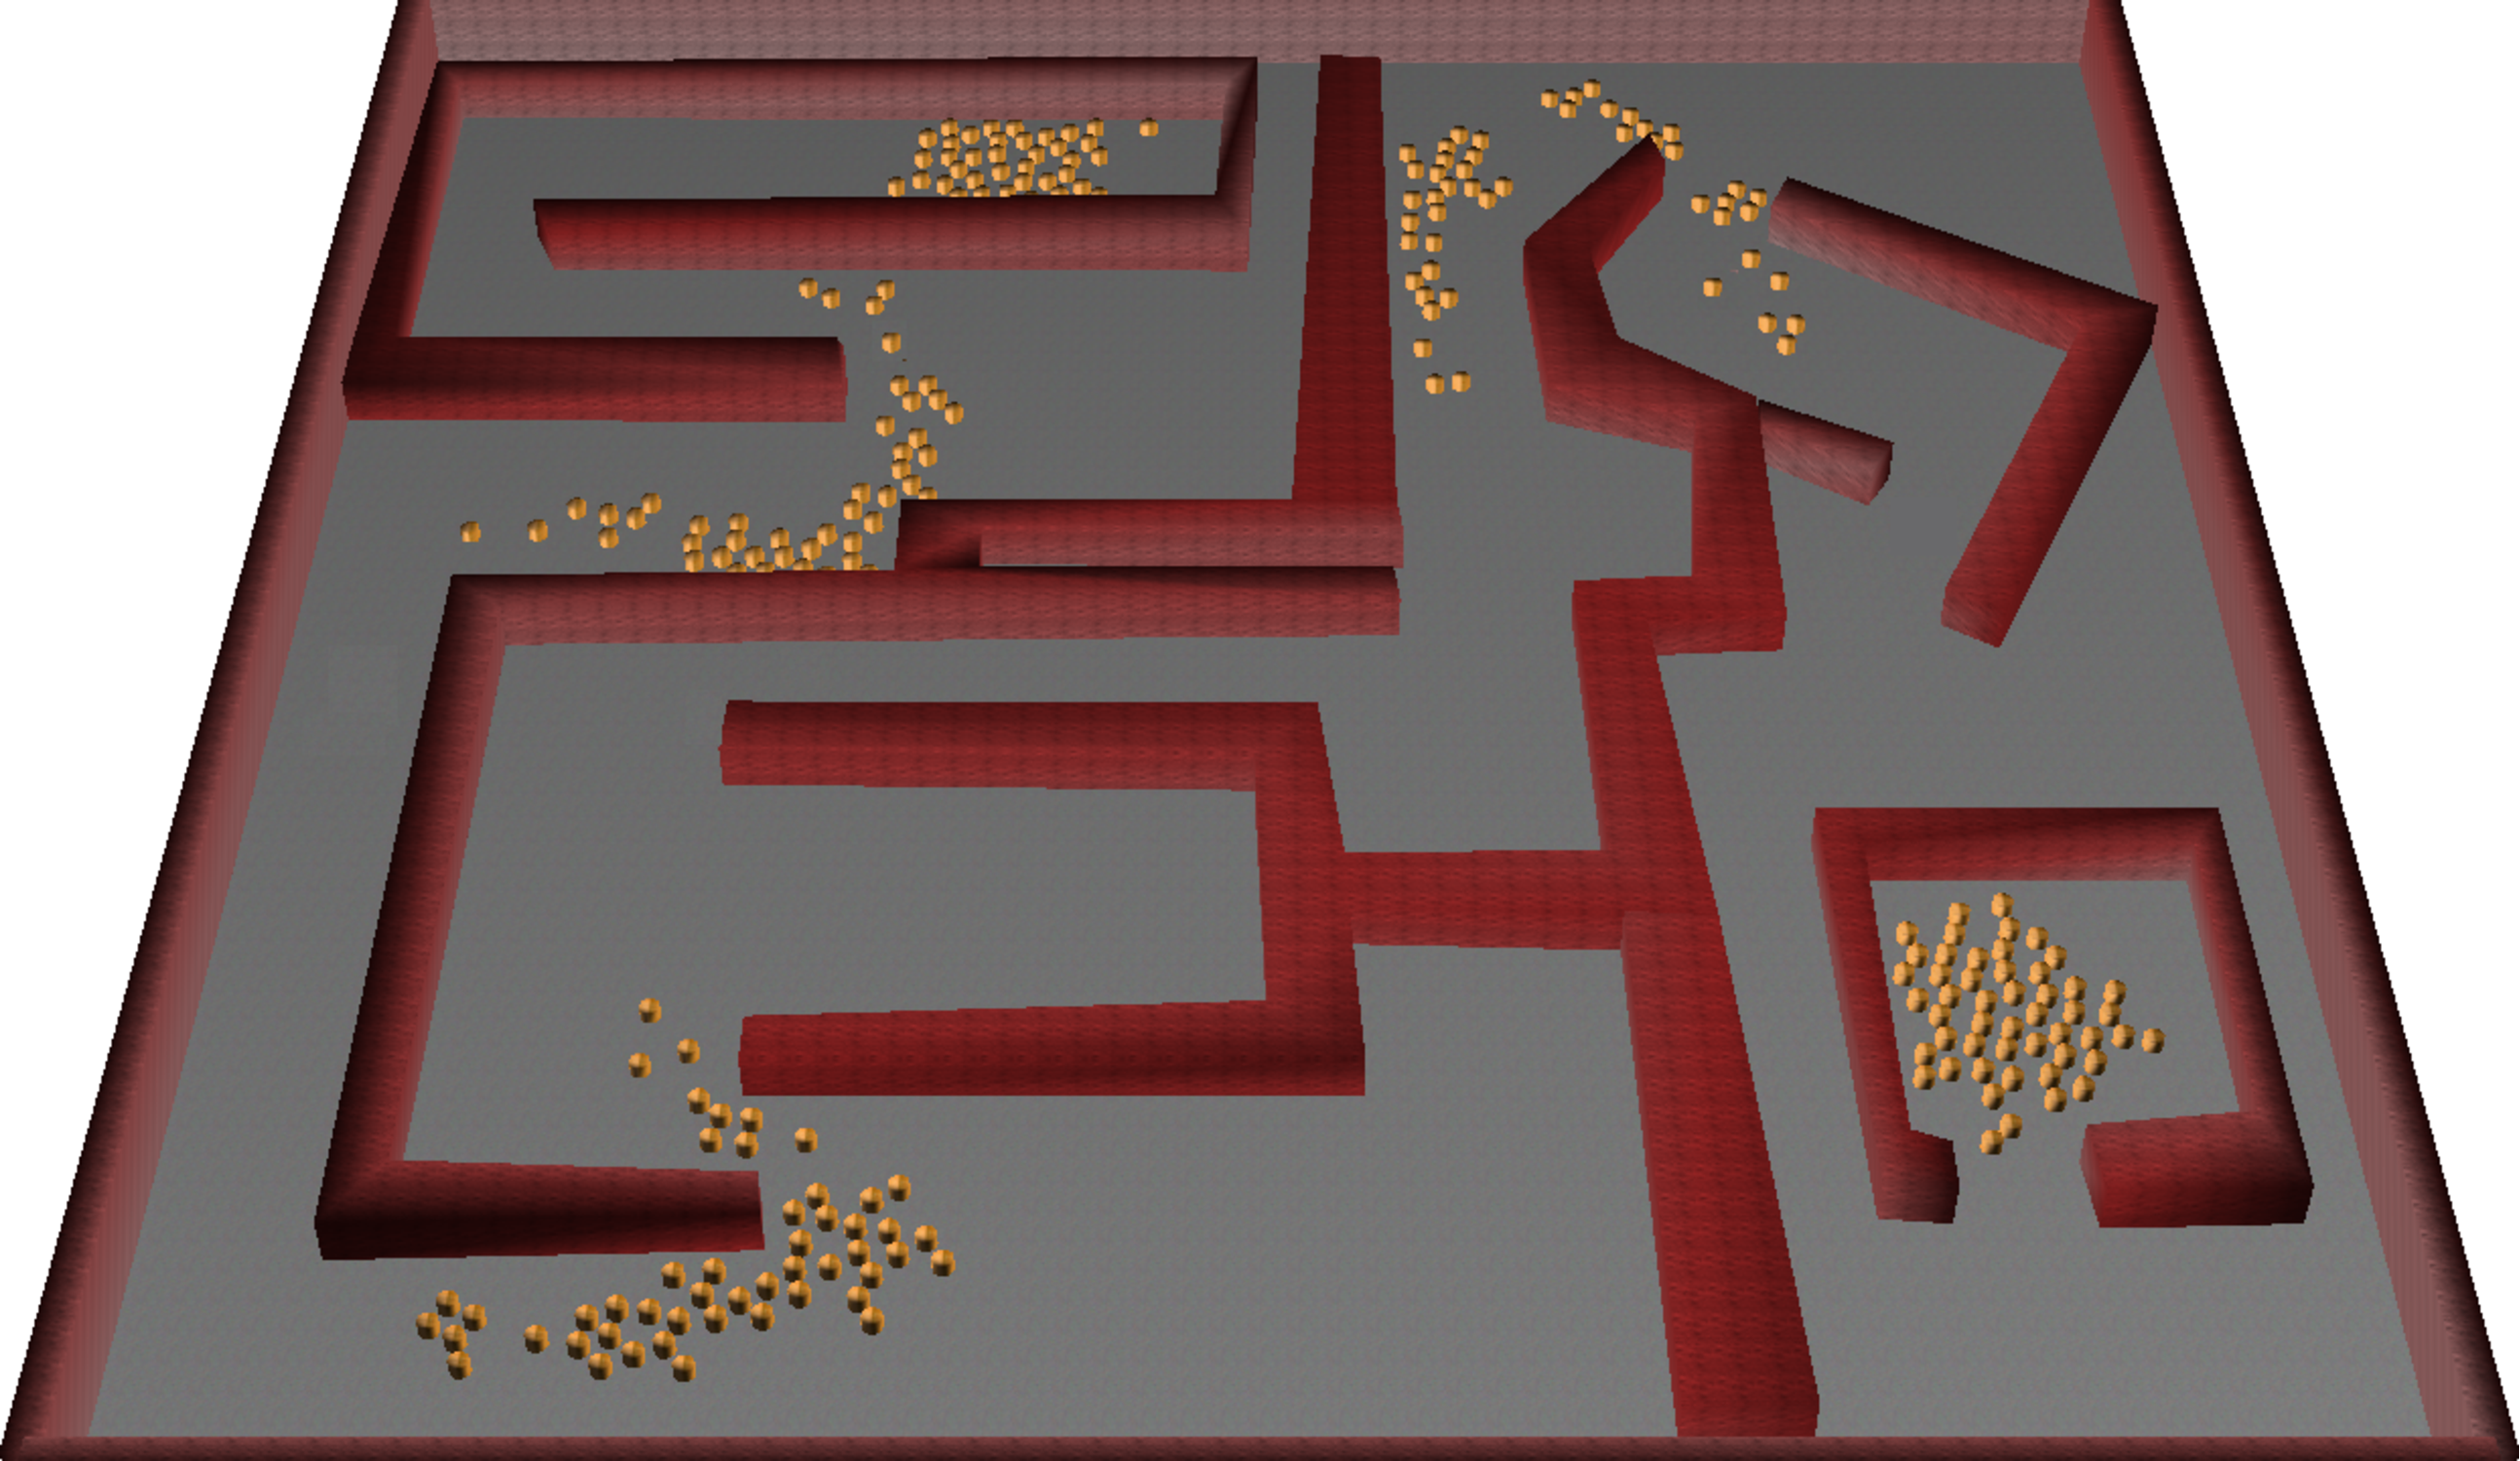
\includegraphics[width=0.55\textwidth]{scene2}}\\
\multicolumn{2}{c}{(c) scene3}
\end{tabular}
\caption{Scenes used in the experiments. Each figure also shows
  intermediate swarm configurations along the path from the initial to
the goal.} 
\label{fig:Scenes}
\end{figure}

\subsection{Measuring Performance}
\label{sec:Measures}
A problem instance is defined by a scene and the number of robots. Due
to the probabilistic nature of the roadmap, performance on a
particular problem instance is based on twenty different runs.
Results report the average time for all the robots to reach the final
destination. Results also report the average distance among all the
robot pairs. More specifically, the average distance for a problem instance is measured by
adding all the pairwise distances at every time step for all the runs
to a vector and then diving by the size of the vector. Finally, the
average distance is scaled by the robot diameter. As an example, a
scaled distance of $5.14$ indicates that the swarm is maintaining an average
separation distance of roughly $5$ robots.  Small values (close to $1$)
indicate that the robots are too close to one another and large values
indicate that the robots are separating. Standard deviations are shown
for both time and scaled distance results.

%$$
%\sum_{run=1}^{20}\sum_{t}
%\left(\sum_{\stackrel{b_i, b_j \in \Var{Robots}}{b_i \neq b_j}}
%||\Var{pos}_t(b_i), \Var{pos}_t(b_j)||_2\right)
%$$

Experiments are conducted on an Intel Core i3 machine (CPU: 2.40GHz,
RAM: 4GB) using Ubuntu 13.04. Code is written in Python 2.7.3. Code is
publicle available at \cite{CodeBoids}.

\subsection{Results}
\label{sec:Results}

Fig.~\ref{fig:ResT}(a) provides a summary of the results on the
average time for all the robots to reach the final
destination. These results indicate that $\Name$ is capable of
effectively planning motions for large swarms moving through
complicated environments. Fig.~\ref{fig:ResT}(b) takes a closer
look at these results by showing how
the average time scales as a function of the number of robots in the
swarm. As the results indicate, the time grows only linearly. Such
results provide promising validation on the scalability of $\Name$. 

\begin{figure}
\centering
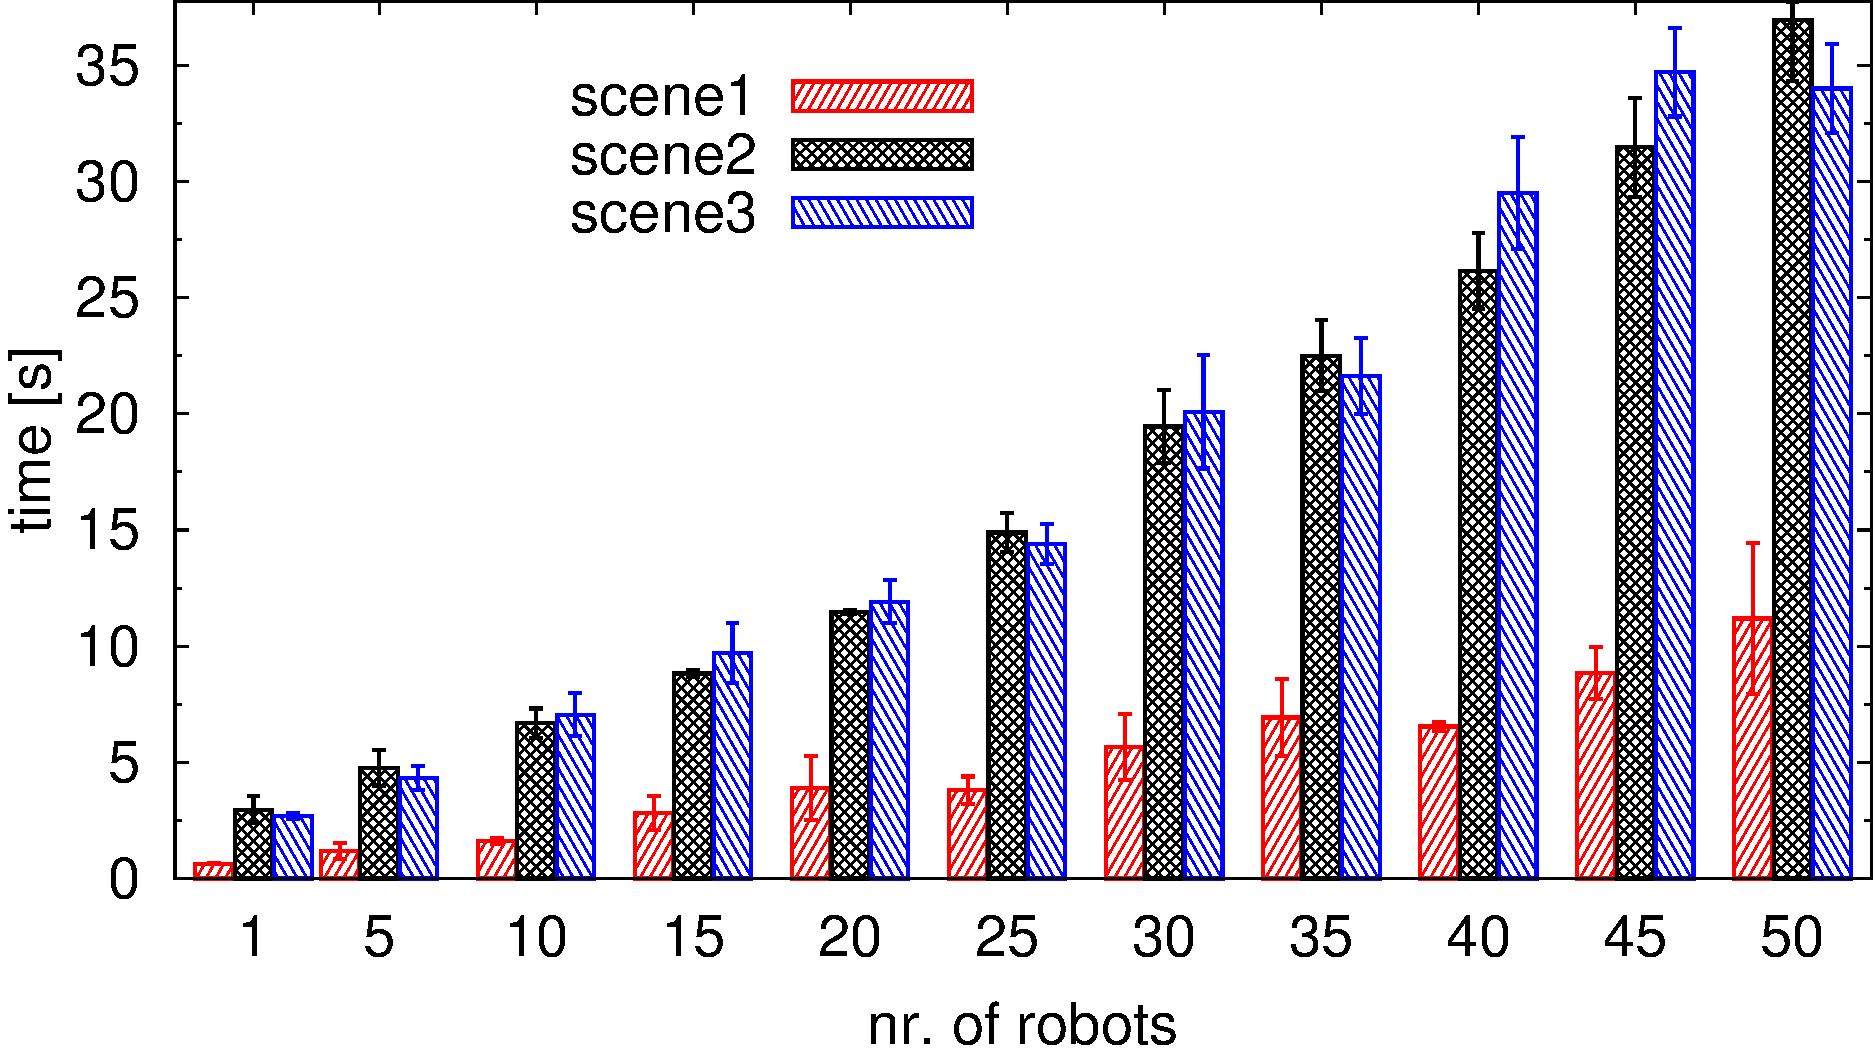
\includegraphics[width=0.49\textwidth]{figResT}
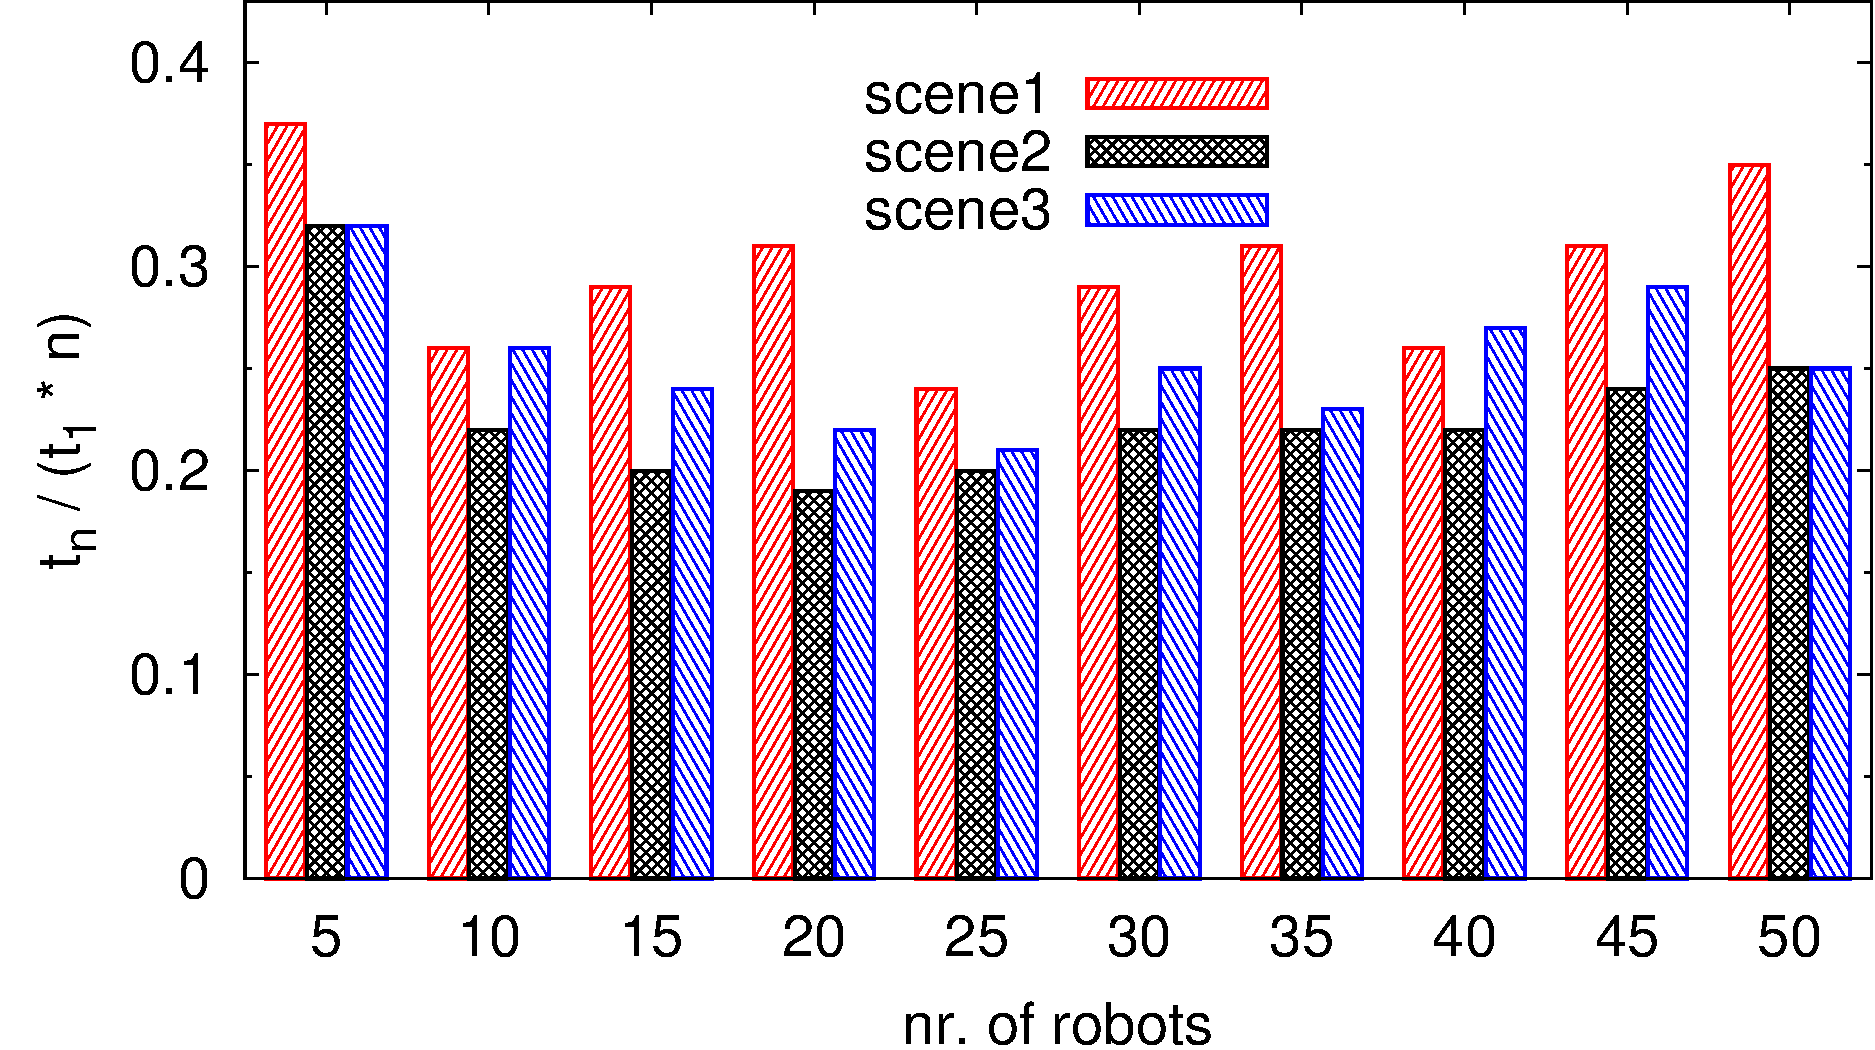
\includegraphics[width=0.49\textwidth]{figResST}
\caption{(a) Results on the average time for all the robots to reach the
  final destination as a function of the number of robots. Bars
  indicate one standard deviation. (b) Scaled results, where $t_n$
  denotes the average time for all $n$ robots to reach the final destination.}
\label{fig:ResT}
\end{figure}

\noindent
The efficiency of $\Name$ derives from the combination of global path
planning via probabilistic roadmaps with local path planning via
potential fields.  To test this further, $\Name$ was run without the
probabilistic roadmap. In this scenario, the robots would be guided by
the potential fields and only be attracted to the final destination
but not to any intermediate goals. Without probabilistic roadmaps,
however, the approach timed out and failed to send any robot to the
final destination. These experiments indicate the importance of
combining probabilistic roadmaps with potential fields when planning
motions for large swarms in complicated environments.


Fig.~\ref{fig:ResFL} shows the average time difference between the
first and the last robot to reach the final destination. The plot
shows that the robots reach the final destination nearly at the same
time even as the number of robots is increased. These results indicate
that the robots remain together and move as a swarm.  



\begin{figure}
\centering
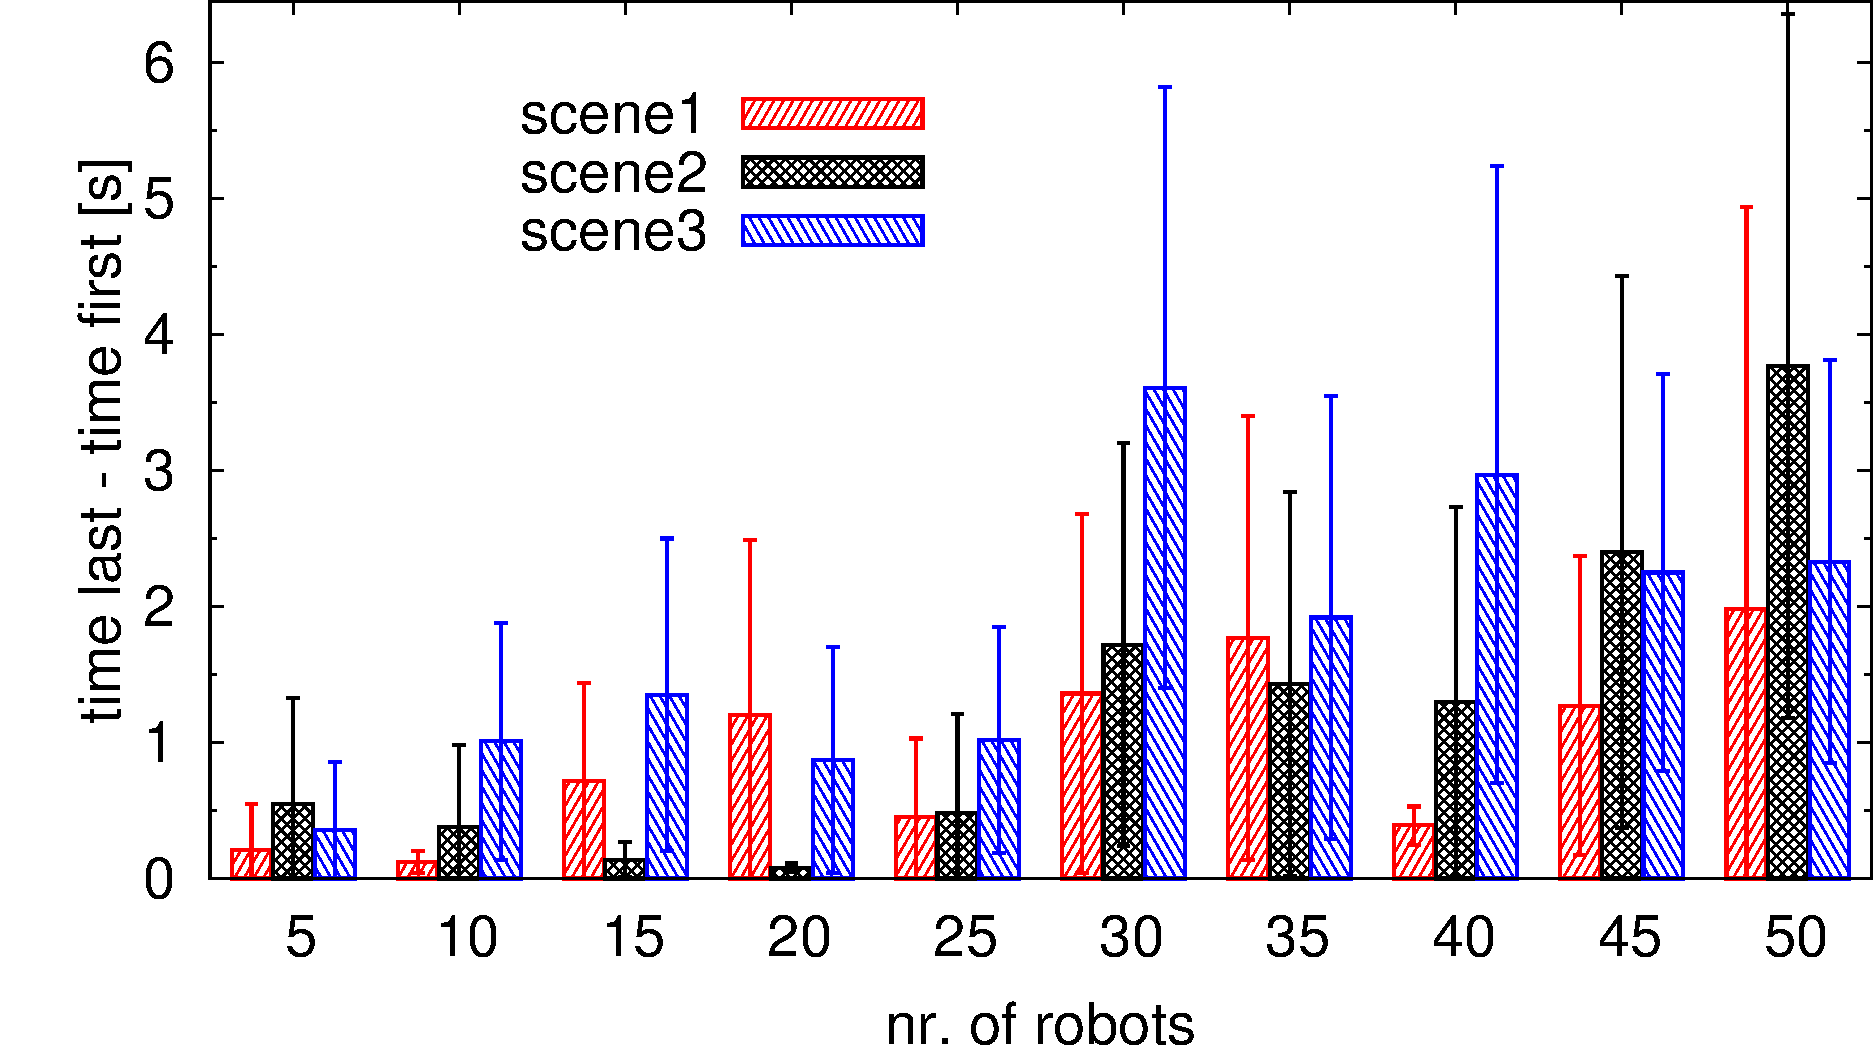
\includegraphics[width=0.65\textwidth]{figResFL}
\caption{Results on the average time difference between the first and
  the last robot to reach the
  final destination as a function of the number of robots. Bars
  indicate one standard deviation.}
\label{fig:ResFL}
\end{figure}

Fig.~\ref{fig:ResD} shows the average scaled distance among all robot
pairs (see Section~\ref{sec:Measures}). The scaled distance provides
an indication of how close the robots are to one another. It is
desirable that the robots are neither too close (as it could cause
collisions or getting stuck in local minima) nor too far from each
other (as it could cause some robots to get separated from the
swarm). The results indicate that the robots maintain a desirable
separation distance. Moreover, the separation distance changes very
little even as the number of robots is increased.

\begin{figure}
\centering
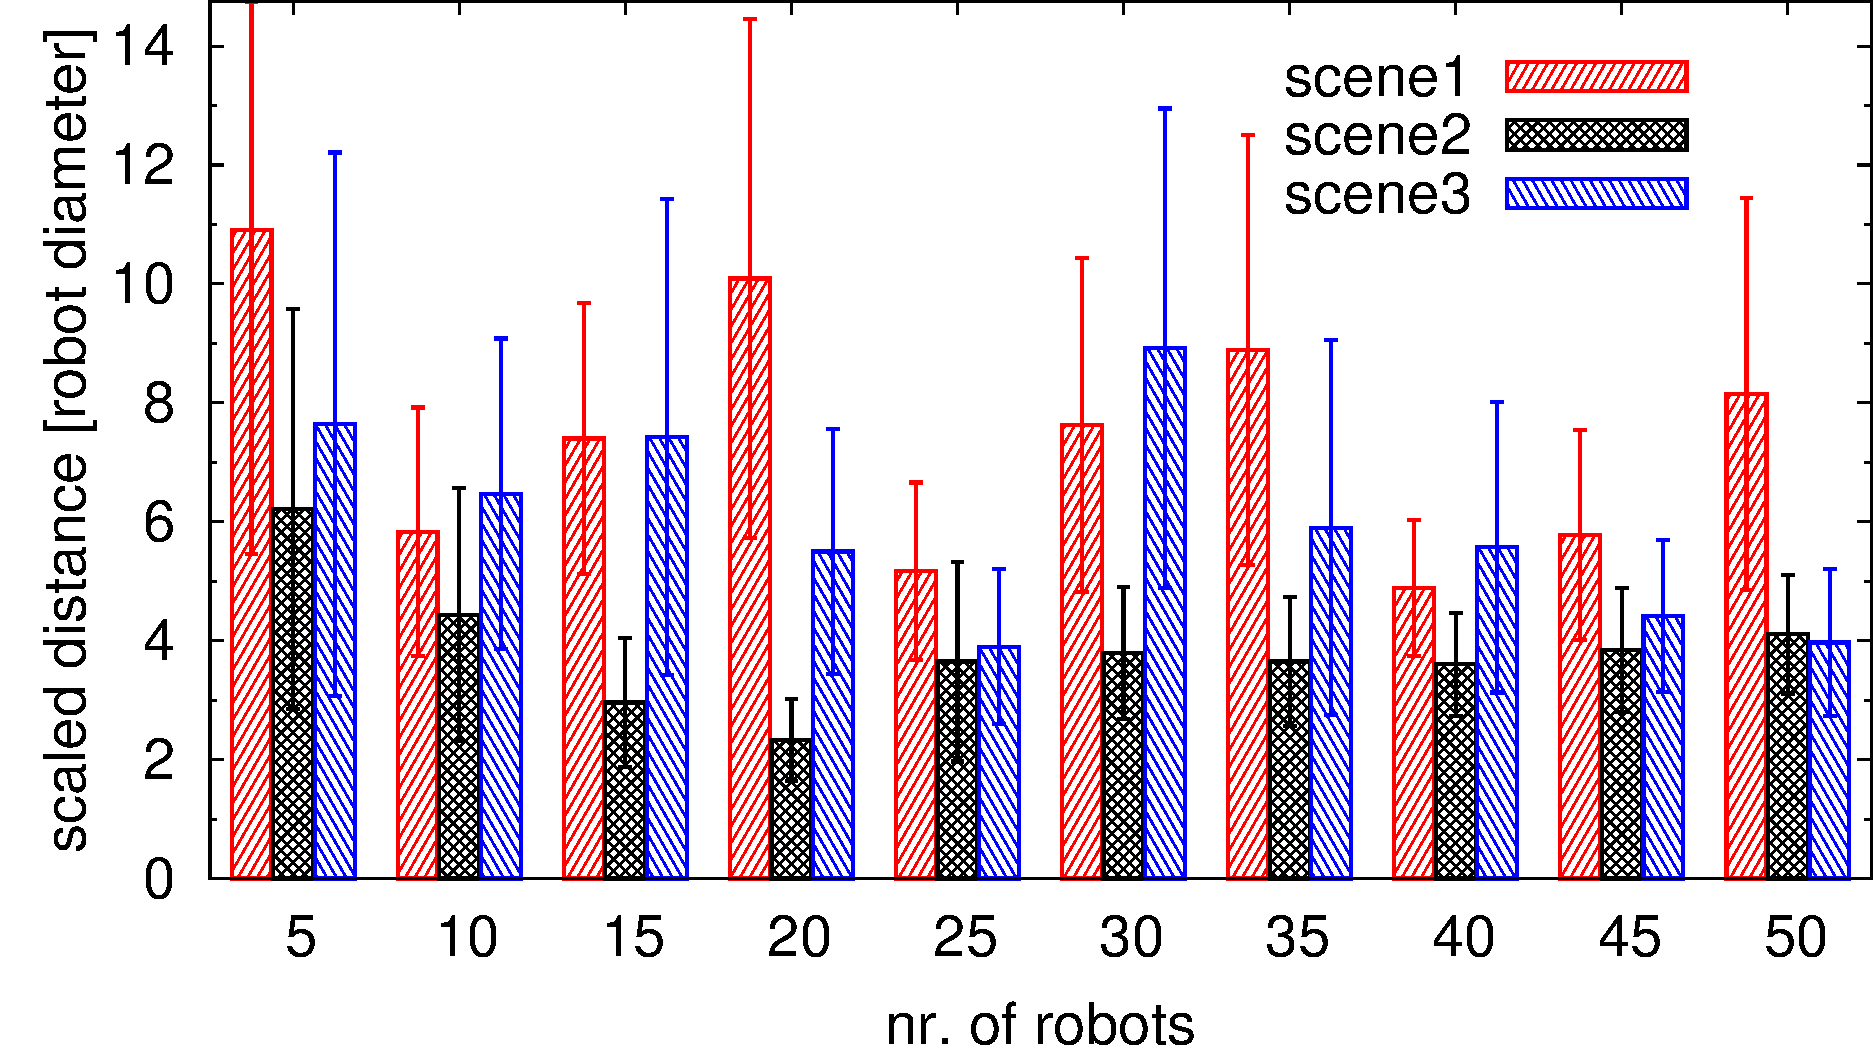
\includegraphics[width=0.65\textwidth]{figResD}
\caption{Results on the average scaled distance among all robot pairs
  as a function of the number of robots. Scaling is done with respect
  to the robot diameter. Bars
  indicate one standard deviation.}
\label{fig:ResD}
\end{figure}


\section{Discussion}

The proposed approach, $\Name$, combined probabilistic roadmaps with
APFs in order to enable a swarm of robots to effectively move to a
desired destination while avoiding collisions with obstacles and each
other.  The probabilistic roadmap provides global path planning to
determine appropriate intermediate goals for the swarm. The potential
fields provide local planning to enable the robots move together as a
swarm towards the goal while avoiding collisions.

The combination of probabilistic roadmaps with APFs opens up several
venues for future research. One research direction is to improve the
interplay between the roadmap planning and APFs in order to more
effectively move the swarm to the desired destination. Another
research direction is to accommodate moving obstacles. As the motion
direction and velocity of the moving obstacles might not be known in
advance, it will be important to be able to predict such motions
and take them into account during planning.



\bibliographystyle{splncs}
\bibliography{mp,plaku}
\end{document}
